\section{DAQ Trigger}
In this chapter we describe how to perform muon lifetime measurments. The electronic chain used for the signal processing is shown in Figure \ref{fig::trigger}.
The scintillators are supplied by the bias voltages reported in Table \ref{tab:bt-setup} and the anodic output signals enter the discriminator to reject background events (thresholds are set according to Table \ref{tab:bt-setup} too).
Before entering the trigger system, the discriminator outputs are multiplied by means of a Fan-In/Fan-Out unit, hence the signals from the upper and the lower scintillators are sent to CH0 and CH1 of the digitizer. The rest of the electronic chain is set in order to perform start and stop topologies for the muon decay triggering. 

\begin{figure}[!h]
	\centering
	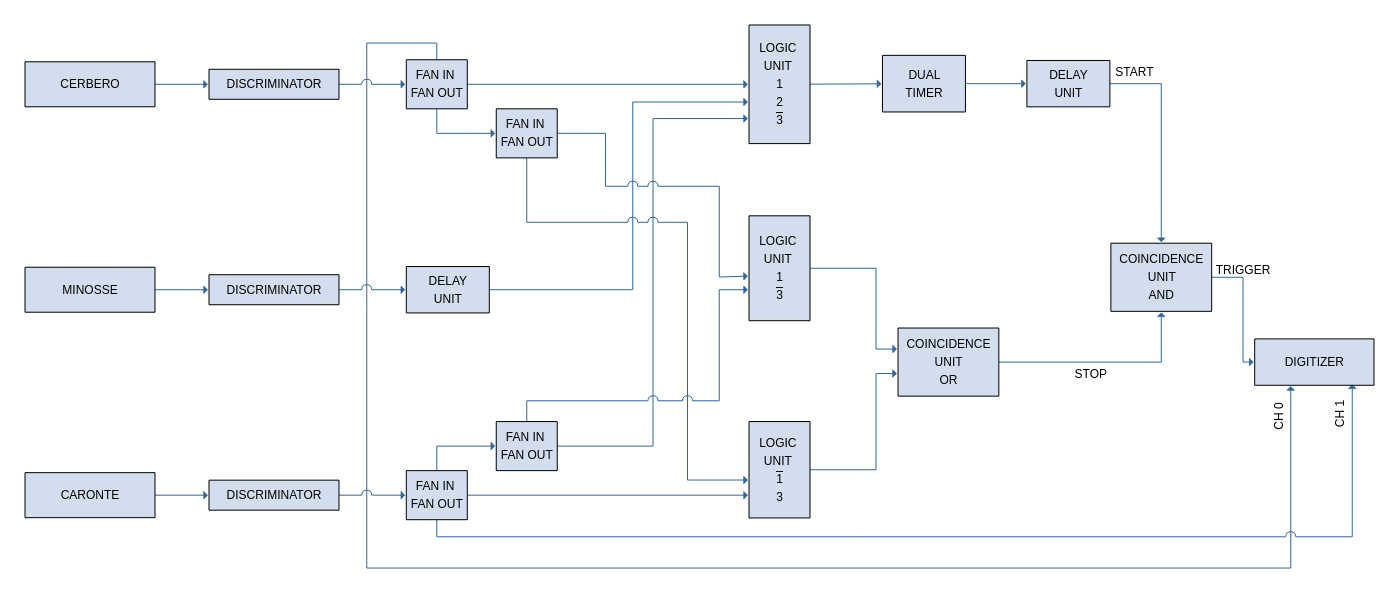
\includegraphics[scale=0.5]{lifetime/trigger}
	\caption{Electronic chain and trigger system used for muon lifetime measurments.}
	\label{fig::trigger}
\end{figure}

\subsection{Trigger system}
To acquire only muon decay events it is necessary to build a trigger system as the one reported in Figure \ref{fig::trigger}, which provides an \emph{external trigger} signal for the digitizer. Therefore the digitizer acquires \emph{Cerbero} and \emph{Caronte} waveforms only for those events which satisfy the trigger requirements.
The trigger signal consists in the logic coincidence (\texttt{AND} operation) between a START and a STOP, marking respectively the decay of the muon in the middle scintillator and the release of energy by the charged decay product in one of the external detectors. Figure \ref{fig::scinti_decay} shows a scheme for a possible muon decay event which gives a START event and its corresponding STOP event in the external scintillators.

\subsection{Start}
The START signal corresponds to the capture of the muon in the middle scintillator. This event involves the release of energy in the upper (1) and in the middle detector (2) but not in the lower one (3). Therefore, the START signal is produced by the $1 \wedge 2 \wedge \overline{3}$ topology.\\

The pulses coming from the scintillators are sent into the discriminator module and its output is multiplied by a Fan-In/Fan-Out. The three signals are sent to a programmable logic unit to perform logic \texttt{AND} operation. 
Using the dual timer the START is widened up to $5 \tau_{\mu} \simeq \SI{11}{\micro s}$, which is the period of time in which we expect the most of the selected muons to decay.  %Hence the apparatus is sensible to time measures in the range $[0, 11] \si{\micro s}$.\\
Note that since all START events satisfies also the STOP topology $1 \wedge \overline{3}$, the START signal is delayed of $\sim \SI{50}{\nano s}$ by means of a delay unit and LEMO cables in order to prevent fake trigger events caused by auto-coincidences.

\begin{figure}[!h]
	\centering
	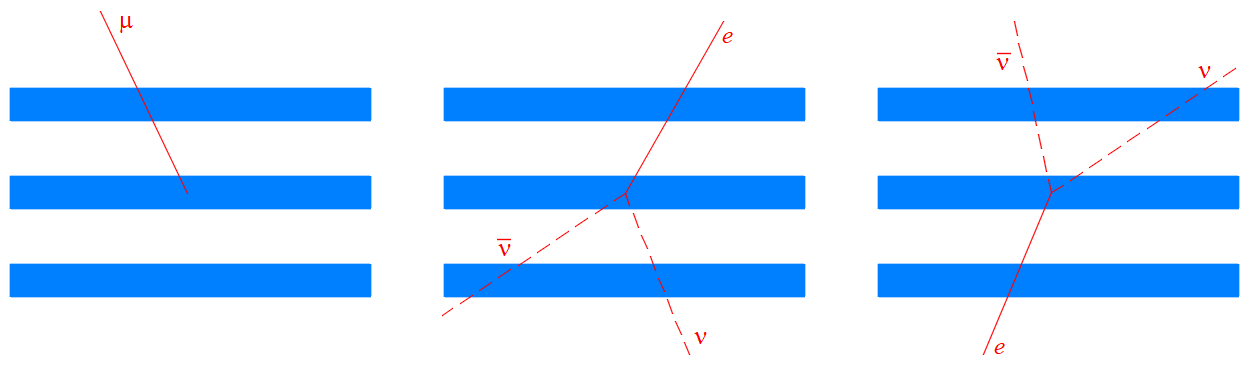
\includegraphics[scale=0.44]{lifetime/scinti_decay}
	\caption{Scheme of a possible muon decay event. The incident muon stops in the middle scintillator (START with $1 \wedge 2 \wedge \overline{3}$ topology). The muon decays releasing energy in the upper or in the lower scintillator (STOP with $1 \land \overline 3$ or $\overline 1 \land 3$ respectively).}
	\label{fig::scinti_decay}
\end{figure}

Actually, the START topology does not guarantee uniquely that a muon decay event has happened. In fact there is also the possibility for a muon to cross 1 and 2 without crossing 3 because of the geometric acceptance (see Figure \ref{start_false}).

\begin{figure}[!thp]
	\centering
	\begin{subfigure}{.3\linewidth}
		\centering
		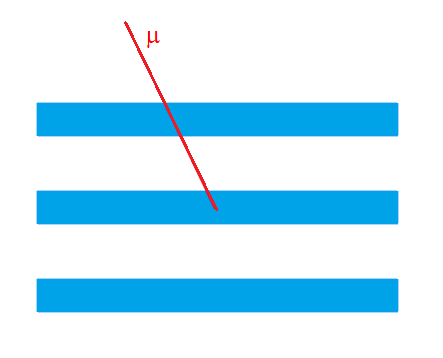
\includegraphics[width=\linewidth]{lifetime/start_true}
		\caption{True START: $\mu$ crosses 1 and 2 stopping in it.}
		\label{start_true}
	\end{subfigure}
	\begin{subfigure}{.3\linewidth}
		\centering
		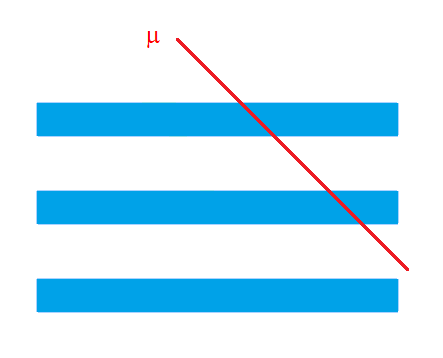
\includegraphics[width=\linewidth]{lifetime/start_false}
		\caption{False START: $\mu$ crosses 1 and 2 without stopping in it.}\label{start_false}
	\end{subfigure}
	\caption{Schemes of true and false START events.}
	\label{}
\end{figure}


\subsection{Stop} 
The STOP signal corresponds to the loss of energy of the charged lepton produced in the decay in one of the outer scintillators. To produce the STOP signal a programmable logic unit is used to perform an \texttt{AND} operation between the signals from the external detectors. In this way it is possible to select only event topologies corresponding to a charged lepton which crosses the upper scintillator and not the lower one ($1 \wedge \overline 3$) or vice versa ($\overline 1 \wedge 3$). The output of these logic operations are sent into a coincidence unit performing an \texttt{OR} operation between the two STOPs, obtaining the overall STOP topology $ (1 \land \overline 3) \lor (\overline 1 \land 3) $.
Finally, a logical \texttt{AND} is performed between the overall STOP and the widened and delayed START signals.\\
Note that false STOP events could happen due to the detectors geometric acceptance. Nevertheless these STOP events are less probable as they are suppressed by the $\cos^{2} \theta$ angular distribution. Figure \ref{false_stop_events} shows some examples of possible false STOP events.


\begin{figure}[!thp]
	\centering
	\begin{subfigure}{.26\linewidth}
		\centering
		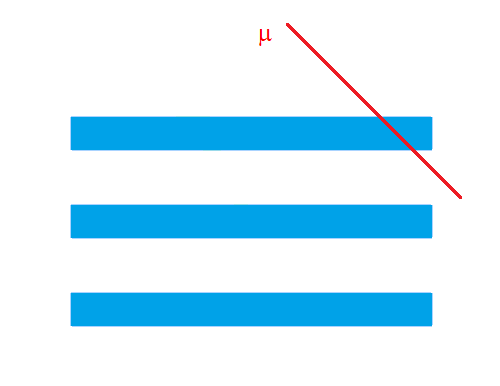
\includegraphics[width=\linewidth]{lifetime/falso_stop}
		\caption{False $ (1 \land \overline 3)$ STOP.}
		\label{false_stop}
	\end{subfigure}
	\begin{subfigure}{.26\linewidth}
		\centering
		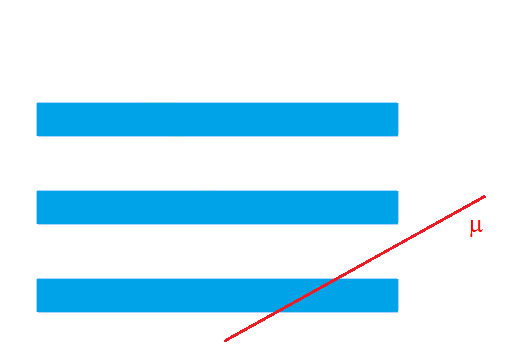
\includegraphics[width=\linewidth]{lifetime/falso_stop_2}
		\caption{False $ (\overline 1 \land  3)$ STOP.}
		\label{false_stop_2}
	\end{subfigure}
	\begin{subfigure}{.26\linewidth}
		\centering
		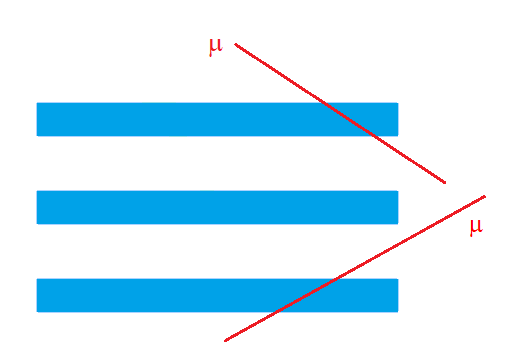
\includegraphics[width=\linewidth]{lifetime/falso_stop_3}
		\caption{False $ (1 \land \overline 3) \lor (\overline 1 \land 3) $ STOP.}
		\label{false_stop_3}
	\end{subfigure}
	\caption{Schemes of possible false STOP events.}\label{false_stop_events}
\end{figure}

\subsection{Further observations} \label{obs}
Since the trigger system has been built using many electronic modules and different cables, it is of primary importance to keep under control all the delays introduced during the configuration of the electronic chain. For this reason, during the construction of the trigger system, the input-output delays of each module have been taken into account and LEMO cables of suitable length have been used in order to have signals which reach the programmable logic unit gates all with the same delay.\\
%In Figure \ref{fig:osc_coinc} is shown the oscilloscope visualization of the START and STOP signals which enter the final Coincidence Unit in \texttt{AND} mode and whose coincidence gives the trigger signal. Note that in Fig. \ref{subfig::strat_stop_delay} the START signal has been conveniently delayed respect to the STOP signal in order to prevent fake coincidences (i.e. START autocoincidences). The STOP signal outgoing the logic $\texttt{OR}$ gate exhibits a double square pulse which is due to signal rebouincing and can be prevented widening the gate width of the Coincidence Unit in $\texttt{OR}$ mode up to $\sim \SI{100}{ns}$.  In Figure \ref{subfig::eccoilmu} is shown the evidence of a muon decay event given by the coincidence of the START and STOP signals. Note how the use of the Dual Timer to extend the start signal up to $\SI{11}{\micro s}$ is necessary to detect muon decay events.\\
%\begin{figure}[!htp]
%	\centering
%	\begin{subfigure}{.45\linewidth}
%		\centering
%		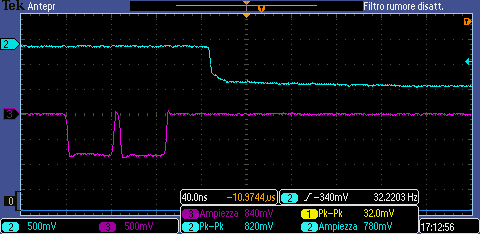
\includegraphics[width=\linewidth]{lifetime/TEK00002}
%		\caption{The START signal is delayed to prevent fake coincidences. }
%		\label{subfig::strat_stop_delay}
%	\end{subfigure}\hfill
%	\begin{subfigure}{.45\linewidth}
%		\centering
%		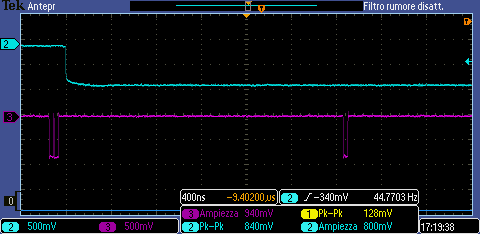
\includegraphics[width=\linewidth]{lifetime/TEK00003}
%		\caption{Evidence of a muon decay given by an $\texttt{AND}$ coincidence between the START and STOP signal.}
%		\label{subfig::eccoilmu}
%	\end{subfigure}
%	\caption{Oscilloscope visualization. The white line represents the START signal while purple line represents the STOP signal outgoing the Coincidence Unit in \texttt{OR} mode.}
%	\label{fig:osc_coinc}
%\end{figure}

Figure \ref{fig:fin} shows the oscilloscope visualization of the anodic output of \emph{Cerbero}, its discriminator output and the programmable logic unit $1 \land \overline{3}$ output signal. In Subsection \ref{discriminator} \emph{Cerbero} discriminator width was set to $\SI{80}{\nano s}$ in order to prevent false double or triple counts due to the considerable noise fluctuations. In this case, since \emph{Cerbero} discriminator output is twice the \emph{Caronte} one, the effect is to get multiple STOPs given by the fake coincidences of different signals detected in \emph{Caronte} within the discriminator width of a single \emph{Cerbero} signal.
For this reason, \emph{Cerbero} discriminator width has been restricted up to $\SI{57.6}{\nano s}$.


\begin{figure}[!htp]
	\centering
	\begin{subfigure}{.45\linewidth}
		\centering
		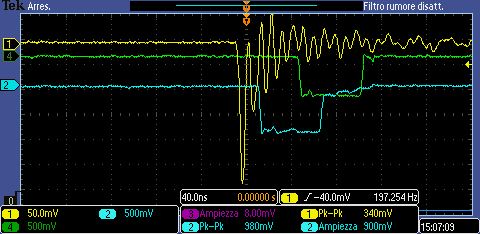
\includegraphics[width=\linewidth]{lifetime/TEK00005}
		\caption{Logic coincidence $1 \land \overline 3$.}
	\end{subfigure}\hfill
	\begin{subfigure}{.45\linewidth}
		\centering
		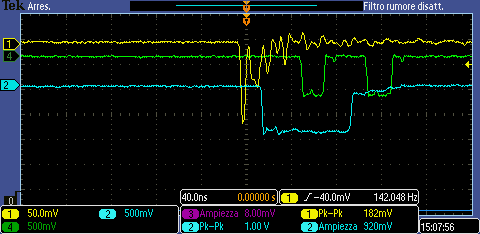
\includegraphics[width=\linewidth]{lifetime/TEK00006}
		\caption{Fake logic coincidence $1 \land \overline 3$.}
	\end{subfigure}
	\caption{Oscilloscope visualization. The yellow line represents \emph{Cerbero} anodic output, the blue line is the discriminator output and the green line represents the programmable logic unit $1 \land \overline{3}$ output signal.}
	\label{fig:fin}
\end{figure}

\section{DAQ software}
\label{DAQ}
Events data acquisition is performed thanks to the CAEN Digitizer. In particular, pulses\footnote{The Digitizer requires standard NIM inputs, thus the two incoming signals are taken after the discrimination stage.} from the upper detector and the lower one are sent to Digitizer channels 0 and 1, respectively and they are actually acquired only when the external trigger green-lights it.\\

Digitizer saves events by using \texttt{.XML} format, which means \emph{eXstensible Markup Language}. The extend-ability of this language is given by the possibility to define personalized tags, extremely useful in order to organize data within a specific logic. Hence, after a prior analysis of the \texttt{XML} structure, a parser based on \texttt{BeautifulSoup4 Python} library has been developed (see Appendix \ref{app:xml_parser}): each triggered event is stored in a \texttt{ROOT TDirectory} and it consists of two waveforms (channels 0 and 1) saved as \texttt{TGraph}s. The \texttt{XML\_parser} output is given by a \texttt{TFile}. This first step is needed since lifetime measurements collect a lot of thousands of events and a well organized data structure is certainly a plus.\\

The interesting events are distinguished by two pulses: the first one is the passage of a $\mu^\pm$ through the upper scintillator, whilst the second one is caused by the emitted $e^\pm$ and it can be recorded both in the upper or the lower detector. For this reason a first skim that discards all the other types of events has been implemented (Figure \ref{fig:rej} gives two examples of rejected events).\\

The final stage of the DAQ software consists in the computing of the time shifts $\Delta t$ through the two waveforms: instead of fitting the pulses (in a partial range) by means of \emph{Fermi-Dirac}-like functions, a method based on the pulse derivative\footnote{The derivative of a square pulse is a Dirac-$\delta$.} (see Figure \ref{fig:derivative}) is performed due to the smaller computational cost and the distance between peaks is easily obtained.

\begin{figure}[!htp]
	\centering
	\begin{subfigure}{.5\linewidth}
		\centering
		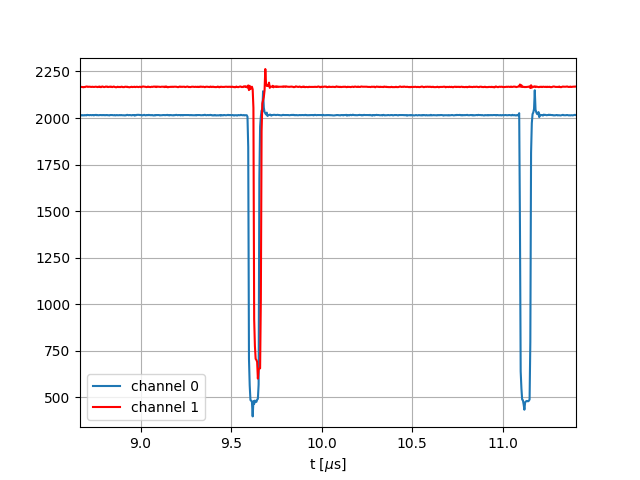
\includegraphics[width=\linewidth]{lifetime/rejected1}
	\end{subfigure}\hfill
	\begin{subfigure}{.5\linewidth}
		\centering
		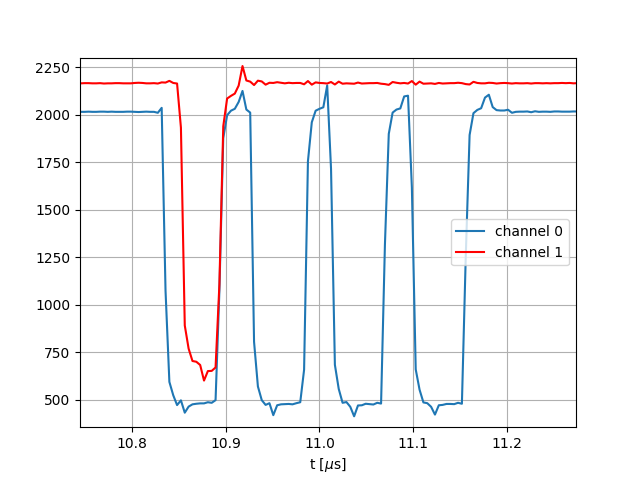
\includegraphics[width=\linewidth]{lifetime/rejected2}
	\end{subfigure}
	\caption{Examples of rejected events.}
	\label{fig:rej}
\end{figure}

\begin{figure}[!htp]
	\centering
	\begin{subfigure}{.5\linewidth}
		\centering
		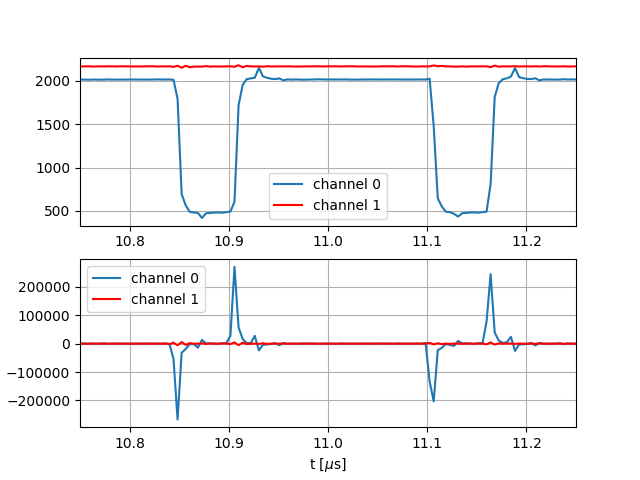
\includegraphics[width=\linewidth]{lifetime/up_decay}
		\caption{Electron/positron emitted towards the\\ upper detector.}
	\end{subfigure}\hfill
	\begin{subfigure}{.5\linewidth}
		\centering
		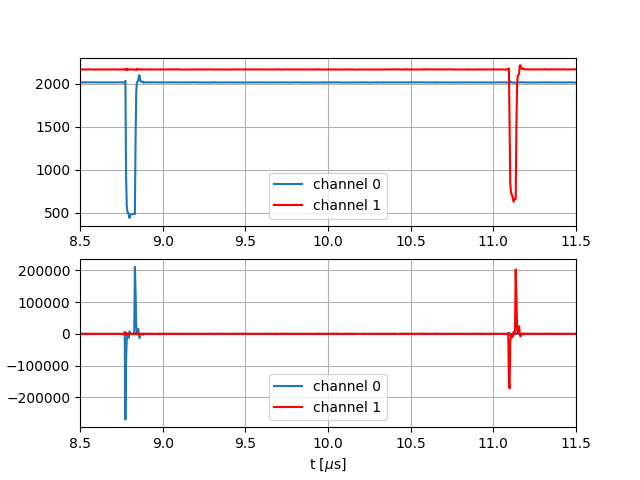
\includegraphics[width=\linewidth]{lifetime/down_decay}
		\caption{Electron/positron emitted towards the\\ lower detector.}
	\end{subfigure}
	\caption{The upper plots represents the waveforms, while the lower plots are their derivatives. The time shift is calculated as the distance between the peaks minimums.} \label{fig:derivative}
\end{figure}

\section{Preliminary studies}
Offline data analyses have been made on the triggered signals: the Digitizer acquires \emph{Cerbero} and \emph{Caronte} waveforms and the DAQ software allows us to distinguish between STOPs in the upper or in the lower detector. A histogram is filled with different $\Delta t$s and what we expect is a negative exponential trend given by

\begin{equation} \label{exp}
N(\Delta t) = N_0\cdot e^{-\Delta t/\tau} + B
\end{equation}
where $\tau$ is the muon lifetime and $B$ is the uniform background due to random coincidences (see Appendix \ref{Background} for further details for the background estimation). 

\subsection{Preliminary lifetime measurements}
A first measurement campaign has been performed with the setup shown in Table \ref{tab:bt-setup}.
\begin{table}[!h]
	\centering
	\begin{tabular}{ccc||ccc}
		\toprule
		Up pulses & Down pulses & $N$ & Up pulses & Down pulses & $N$\\
		\midrule
		\rowcolor{blue!25}$3$&$0$&$1559$ & $2$&$2$&$12$\\
		\rowcolor{blue!25}$2$&$1$&$1307$ & $6$&$1$&$9$\\
		\cellcolor{blue!25}$4$&\cellcolor{blue!25}$0$&\cellcolor{blue!25}$249$ & $0$&$1$&$6$\\
		\rowcolor{blue!25}$3$&$1$&$130$ & $7$&$1$&$4$\\
		\rowcolor{blue!25}$5$&$0$&$72$ & $3$&$2$&$3$\\
		$1$&$2$&$58$ & \cellcolor{blue!25}$7$&\cellcolor{blue!25}$0$&\cellcolor{blue!25}$3$\\
		\rowcolor{blue!25}$4$&$1$&$46$ & $9$&$1$&$2$\\
		\cellcolor{blue!25}$5$&\cellcolor{blue!25}$1$&\cellcolor{blue!25}$30$ & $1$&$3$&$1$\\
		$1$&$0$&$17$ & 	$1$&$1$&$1$\\
		\rowcolor{blue!25}$6$&$0$&$15$ & $8$&$1$&$1$\\
		\bottomrule		
	\end{tabular}
	\caption{Rejected events ($3525$ of $20644$) morphology in the preliminary study \#1. Highlighted rows are related to events with an excess of up pulses.}\label{tab:skim1}
\end{table}
The number of triggered events is $20644$ but $3525$ of them have been rejected by the skim procedure whose results are shown in Table \ref{tab:skim1}, where it is possible to see how the most of rejected events are caused by an excess of upper-detector pulses. This result, together with the bad behavior of the histogram represented in Figure \ref{fig:lt1},
\begin{figure}[!htp]
	\centering
	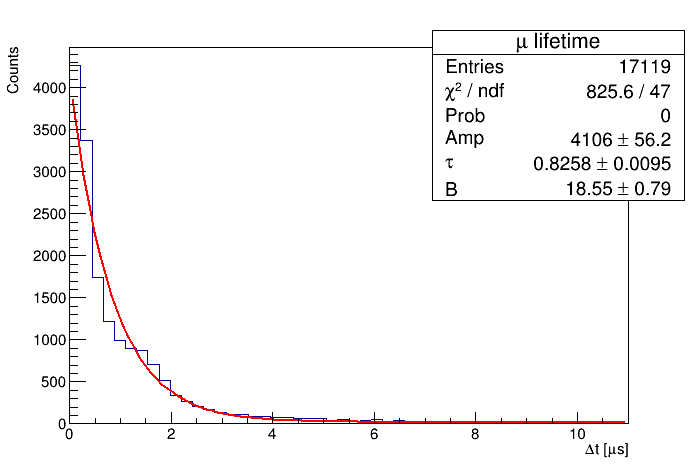
\includegraphics[width=.5\linewidth]{lifetime/lifetime_overall_cerbero40}
	\caption{Overall lifetime preliminary study \#1. \emph{Cerbero} discrimination threshold: $\SI{40}{mV}$.}\label{fig:lt1}
\end{figure}
(where the $p$-value suggests the non-accordance between data and model \eqref{exp}) is a clear sign of problems with the upper scintillator: to prove this statement the  single-rate of \emph{Cerbero} has been measured, giving a result equal to
\begin{equation}
	R\left(\SI{40}{mV}\right) \simeq \SI{116}{Hz}
\end{equation}
which is greater than the expected $\sim\SI{40}{Hz}$.
Thus, the discrimination threshold has been increased to $\SI{70}{mV}$ and a second preliminary measurement has been carried out. Table \ref{tab:skim2} shows how triggered non-physical events (that have been rejected) decrease from $17\,\%$ to $10\,\%$.
\begin{table}[!h]
	\centering
	\begin{tabular}{ccc||ccc}
		\toprule
		Up pulses & Down pulses & $N$ & Up pulses & Down pulses & $N$\\
		\midrule
		\cellcolor{blue!25}$2$&\cellcolor{blue!25}$1$&\cellcolor{blue!25}$756$ & $0$&$1$&$16$\\
		\rowcolor{blue!25}$3$&$0$&$337$ & $5$&$0$&$15$  \\
		$1$&$2$&$166$ & \cellcolor{blue!25}$5$&\cellcolor{blue!25}$1$&\cellcolor{blue!25}$13$  \\
		\rowcolor{blue!25}$3$&$1$&$119$ & $3$&$2$&$4$  \\
		\cellcolor{blue!25}$4$&\cellcolor{blue!25}$1$&\cellcolor{blue!25}$54$ & $1$&$3$&$3$\\
		\rowcolor{blue!25}$4$&$0$&$47$ & $6$&$1$&$1$\\
		\rowcolor{blue!25}$2$&$2$&$28$ & $4$&$2$&$1$\\
		$1$&$0$&$18$ &&&\\
		\bottomrule		
	\end{tabular}
	\caption{Rejected events ($1578$ of $16407$) morphology in the preliminary study \#2. Highlighted rows are related to events with an excess of up pulses.}\label{tab:skim2}
\end{table}
\begin{figure}[!htp]
	\centering
	\begin{subfigure}{.5\linewidth}
		\centering
		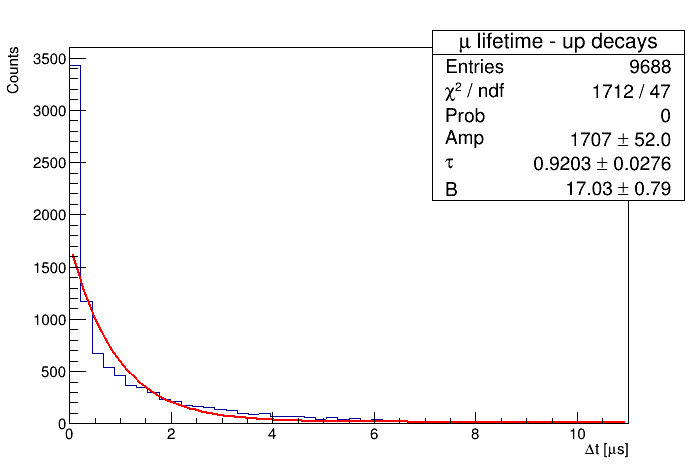
\includegraphics[width=\linewidth]{lifetime/lifetime_up_cerbero70}
		\caption{Up decays.}\label{subfig:lt2up}
	\end{subfigure}
	\begin{subfigure}{.5\linewidth}
		\centering
		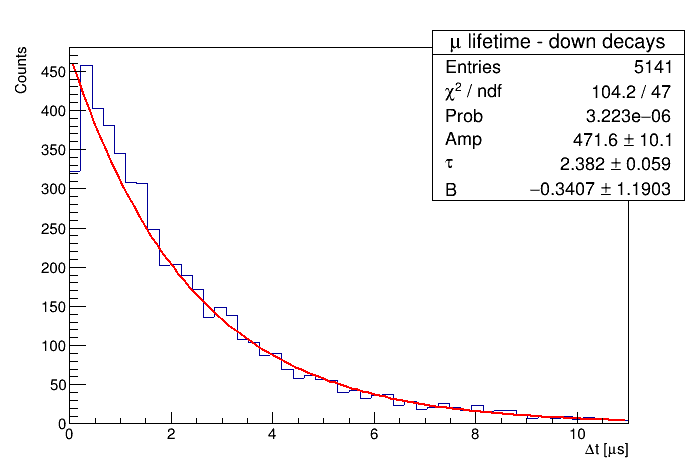
\includegraphics[width=\linewidth]{lifetime/lifetime_down_cerbero70}
		\caption{Down decays.}\label{subfig:lt2down}
	\end{subfigure}
	\caption{Lifetime preliminary study \#2. \emph{Cerbero} discrimination threshold: $\SI{70}{mV}$.}\label{fig:lt2}
\end{figure}
Figure \ref{fig:lt2} shows an unexpected asymmetry between up and down decays but this is mainly due to the excess of counts in the first bins of the histogram represented in Figure \ref{subfig:lt2up}. For this reason, we are going to exclude the first bins from the following fit procedures.
However, both up and down decays measured data are not accordant with the model \eqref{exp} and \emph{Cerbero} discrimination threshold has been increased to $\SI{79}{mV}$ in order to reach a single-detector counting rate equal to $\sim\SI{40}{Hz}$ (at the expense of the detection efficiency).
\begin{table}[!htp]
	\centering
	\begin{tabular}{ccc}
		\toprule
		Up pulses & Down pulses & $N$\\
		\midrule
		\rowcolor{blue!25}$2$&$1$&$213$ \\
		\rowcolor{blue!25}$3$&$0$&$101$ \\
		$1$&$2$&$77$ \\
		\rowcolor{blue!25}$3$&$1$&$44$ \\
		\rowcolor{blue!25}$4$&$1$&$22$ \\
		\rowcolor{blue!25}$4$&$0$&$13$ \\
		\rowcolor{blue!25}$2$&$2$&$10$\\
		$1$&$3$&$4$\\
		$0$&$1$&$4$\\
		$1$&$0$&$3$\\
		\rowcolor{blue!25}$5$&$1$&$3$\\
		\rowcolor{blue!25}$3$&$2$&$1$\\
		\bottomrule		
	\end{tabular}
	\caption{Rejected events ($495$ of $6134$) morphology in the preliminary study \#3. Highlighted rows are related to events with an excess of up pulses.}\label{tab:skim3}
\end{table}
\begin{figure}[!htp]
	\centering
	\begin{subfigure}{.5\linewidth}
		\centering
		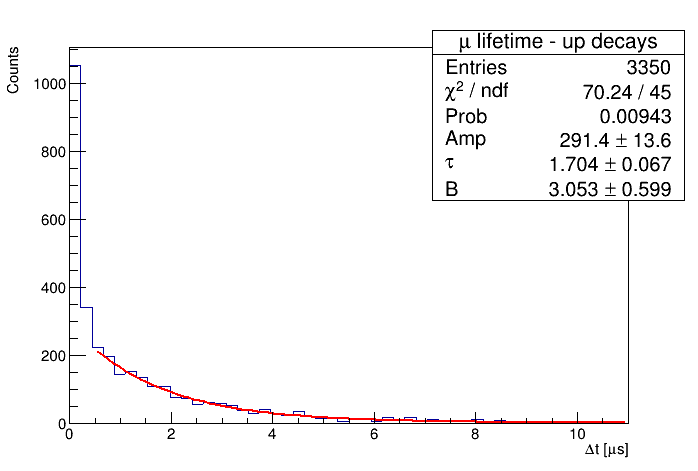
\includegraphics[width=\linewidth]{lifetime/lifetime_up_cerbero79}
		\caption{Up decays.}\label{subfig:lt3up}
	\end{subfigure}\hfill
	\begin{subfigure}{.5\linewidth}
		\centering
		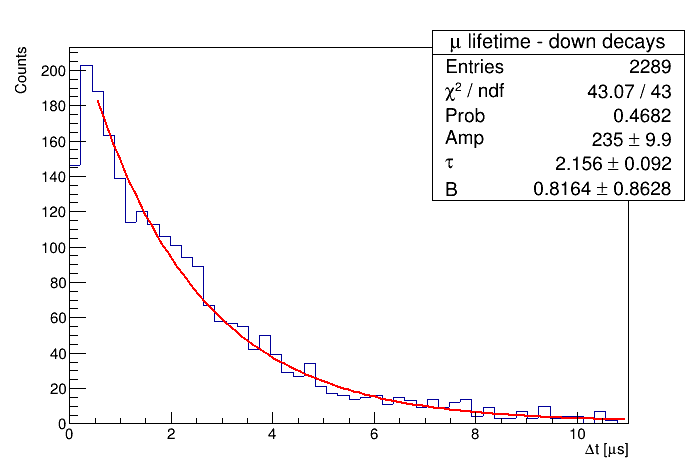
\includegraphics[width=\linewidth]{lifetime/lifetime_down_cerbero79}
		\caption{Down decays.}\label{subfig:lt3down}
	\end{subfigure}
	\begin{subfigure}{.5\linewidth}
		\centering
		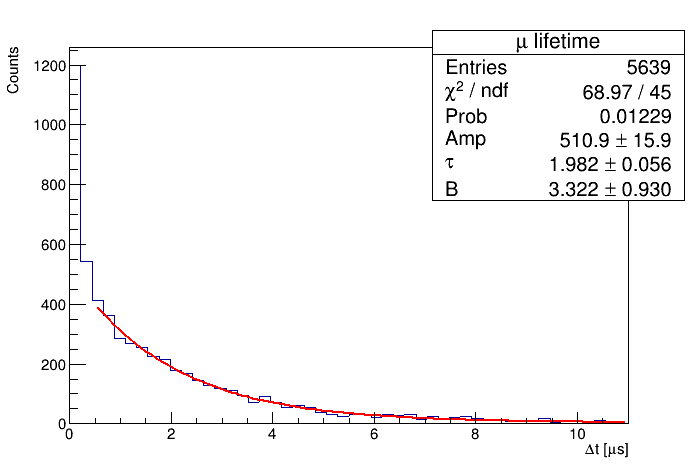
\includegraphics[width=\linewidth]{lifetime/lifetime_overall_cerbero79}
		\caption{Overall decays.}\label{subfig:lt3}
	\end{subfigure}
	\caption{Lifetime preliminary study \#3. \emph{Cerbero} discrimination threshold: $\SI{79}{mV}$. Fit performed by means of the least squares method in the range $[0.5, 11.0]\, \si{\micro \second}$. The number of bins is $50$.}\label{fig:lt3}
\end{figure}
Table \ref{tab:skim3} displays the skim results, highlighting once again that most of the problems are coming from the upper scintillator. Taking into consideration the down decays, a good accordance with the model is observed, in fact the $p$-value is about $47\,\%$ (see Figure \ref{subfig:lt3down}). Notwithstanding the good result obtained in down decays measurements, the bad behavior of the up-like measures (see Figure \ref{subfig:lt3up}) affects the overall histogram shown in Figure \ref{subfig:lt3}.\\

Moreover, by excluding the first bins counts, the asymmetry between the number of up and down decays decreases further.
\begin{table}[!htp]
	\centering
	\begin{tabular}{cccc}
		\toprule 
		\emph{Cerbero} discrimination & Fraction of &Fraction of&Fraction of\\
		threshold (mV) & rejected events & up decays & down decays\\
		\midrule
		$40$ & $0.17$ & $0.88$ & $0.12$\\
		$70$ & $0.10$ & $0.65$ & $0.35$\\
		$79$ & $0.08$ & $0.59$ & $0.41$\\
		\bottomrule
	\end{tabular}
	\caption{Summary of the preliminary study results.}
\end{table}


\subsection{Monte Carlo estimation of the expected lifetime}\label{sec:lifetimeMC}

Since our experimental setup can not distinguish between $\mu^+$ and $\mu^-$ we expect to measure an intermediate lifetime in \emph{carbon} between $\tau_{\mu^+} = \SI{2197}{\nano s}$ and $\tau_{\mu^-} = \SI{2026}{\nano s}$ \cite{lifetime}.
Therefore, a Monte Carlo simulation is developed in order to estimate the mean lifetime of cosmic rays muons we expect to measure in plastic scintillators.
$N$ events are generated  according to a Poisson distribution with mean value equal to the number of events expected in the dataset.
From the up-to-date precise measurement of the \emph{charge ratio} $\mu^+ / \mu^-$ referred to atmospheric muons at surface, obtained by the CMS experiment,
\begin{equation} \label{mu+-}
1.2766 \pm 0.0032 \, (stat.) \pm 0.0032 \,(syst.) \, \cite{charge}
\end{equation}  
it is possible to estimate the composition of $\mu^+$ and $\mu^-$ in cosmic rays at earth
\begin{equation}
f_{\mu^+} =  ( 56.075 \pm 0.087 ) \% \qquad f_{\mu^-} =  ( 43.925 \pm 0.087 ) \% .
\end{equation}
The measured charge ratio $\mu^{+} / \mu^{-}$ depends on the latitude but, since Geneva and Milan have almost the same latitude, this systematic is neglected and only the systematic given by the measure \ref{mu+-} is considered.
The number of events $N$ is divided into $N_{\mu^+}$ and $N_{\mu^-}$ (according to a Binomial distribution) taking into account the fraction $f_{\mu^+}$ and $f_{\mu^-}$ of $\mu^{\pm}$ in cosmic rays. Then, $N_{\mu^+}$ and $N_{\mu^-}$ events with lifetime $\tau_{\mu^+}$ and $\tau_{\mu^-}$, respectively, are generated according to an Exponential distribution.
A histogram with both kind of events is filled and it is fitted with \eqref{exp} neglecting the background term.
5000 independent simulations have been performed and each time a different lifetime with its uncertainties is obtained.
Figure \ref{fig::tau_mc} shows the overall distribution obtained for $\tau_{MC}$ and how the lifetime is estimated from the mean value of a Gaussian distribution.
Actually, the estimated value is affected by a systematic due to the uncertainty on the percentages of cosmic rays $\mu^-$ and $\mu^+$ composition at ground. This systematic uncertainty is estimated by repeating the simulation with both the input parameters $f_{\mu^+}$ and $f_{\mu^-}$ varied within their uncertainties, i.e. changing one at a time the input parameters in the range $[ f_{\mu} - \sigma_{f_{\mu}}, f_{\mu} + \sigma_{f_{\mu}}]$ both for $\mu^+$ and $\mu^-$ and computing the maximum deviation from the mean value as

\begin{equation}
\sigma_{\tau_{MC}}=\max_k\left| \tau_{MC}^k -\langle \tau_{MC} \rangle\right|
\end{equation}
where $k=1, ..., 3^J$ and $J=2$ is the number of parameters $f_{\mu^{\pm}}$.
Finally the estimated muons lifetime in carbon is given by
\begin{equation}\label{tauMC}
\tau_{MC} = \left[ 2.11793  \pm 0.00015 \, (stat) \pm  0.00833 \, (syst) \right]\, \si{\micro\second}.
\end{equation}
\begin{figure}[!htp]
	\centering
	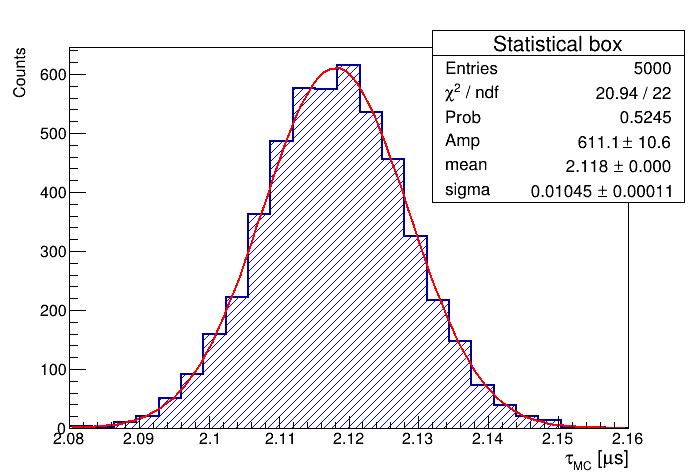
\includegraphics[width=.55\linewidth]{lifetime/tau_mc}
	\caption{Distribution of simulated lifetime $\tau_{MC}$ in carbon and lifetime estimation.}
	\label{fig::tau_mc}
\end{figure}

\section{High statistic lifetime measurement}
Before showing the high statistic measurement, further considerations are needed: first of all, according to what explained in Section \ref{sec:lifetimeMC}, we should better fit the measured distributions with
\begin{equation}\label{2exp}
	N(\Delta t) = N_0^+\cdot e^{-\Delta t/\tau^+} + N_0^-\cdot e^{-\Delta t/\tau^-} + B
\end{equation}
with $N_0^+/N_0^-\simeq 56.1/43.9$, but the fit function \eqref{exp} has been preferred due to $\tau^+$ and $\tau^-$ similarity, in order to simplify the model, i.e. reduce the number of degrees of freedom.

\subsection{Stability check}
The fit procedure relies on least squares method and it has been repeated $800$ times, by varying the number of bins between $50$ and $250$ with a step of $5$ and the fit range between $\SI{6}{\micro\second}$ and $\SI{10.75}{\micro\second}$ with a step of $\SI{0.25}{\micro\second}$. The results of this bi-dimensional study are shown in Figure \ref{fig:stabtau} and \ref{fig:stabchi2}
\begin{figure}[!htp]
	\centering
	\begin{subfigure}{.5\linewidth}
		\centering
		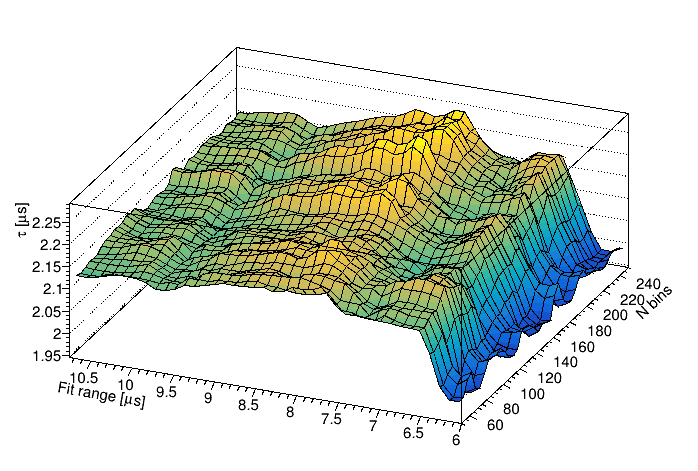
\includegraphics[width=\linewidth]{lifetime/stability_tau3d}
		\caption{3D representation.}
	\end{subfigure}\hfill
	\begin{subfigure}{.5\linewidth}
		\centering
		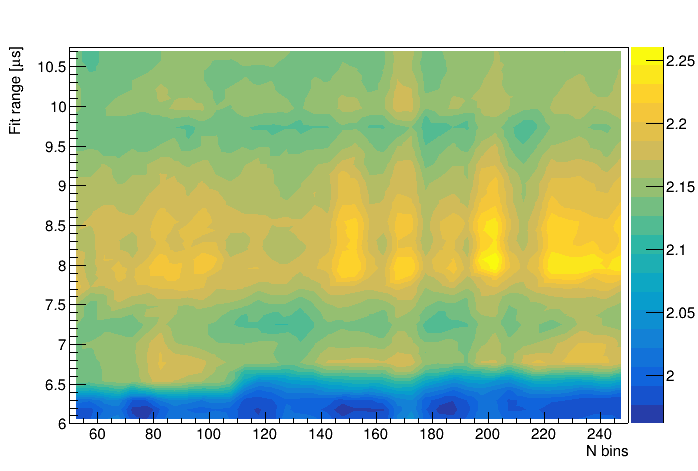
\includegraphics[width=\linewidth]{lifetime/stability_tau}
		\caption{Heat-map.}
	\end{subfigure}
	\caption{Stability check on the estimated $\tau\,\left[\si{\micro\second}\right]$.}\label{fig:stabtau}
\end{figure}
\begin{figure}[!htp]
	\centering
	\begin{subfigure}{.5\linewidth}
		\centering
		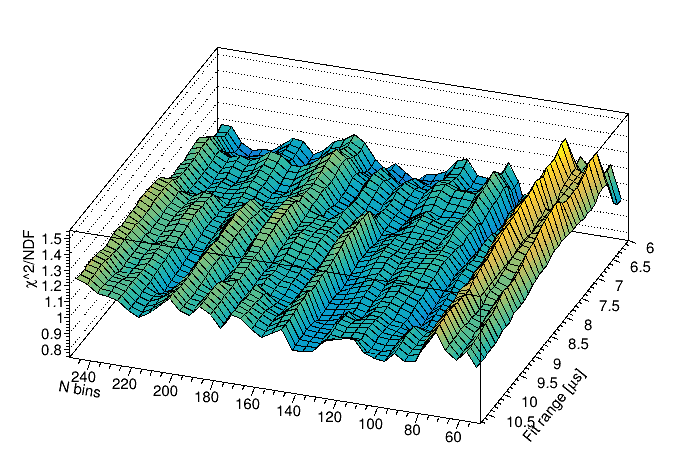
\includegraphics[width=\linewidth]{lifetime/stability_chi23d}
		\caption{3D representation.}
	\end{subfigure}\hfill
	\begin{subfigure}{.5\linewidth}
		\centering
		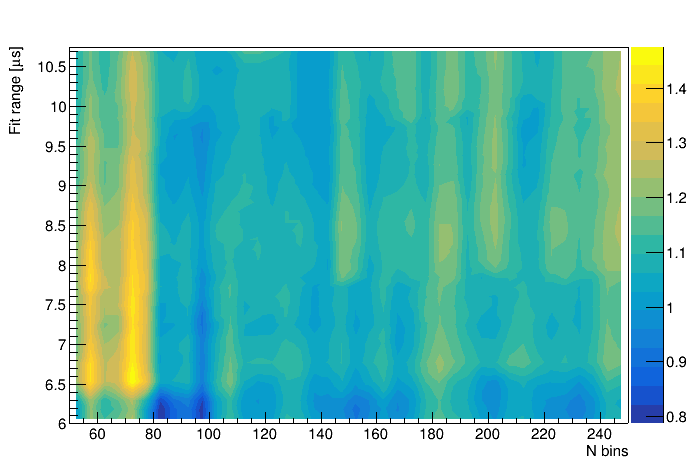
\includegraphics[width=\linewidth]{lifetime/stability_chi2}
		\caption{Heat-map.}
	\end{subfigure}
	\caption{Stability check on the estimated $\chi^2/\textrm{NDF}$.}\label{fig:stabchi2}
\end{figure}
from which we can observe where are the \emph{stability regions}, i.e. portions of the analyzed $\left(\textrm{N bins}, \textrm{Fit range}\,\left[\si{\micro\second}\right]\right)$ space where the estimated $\tau$ and $\chi^2/\textrm{NDF}$ do not vary significantly. A fit range equal to $\SI{10.5}{\micro\second}$ and $100$ bins have been chosen in order to perform the final fit procedure and present the measurement results.


\subsection{Results}\label{subsect::results}

Events are triggered with an observed rate equal to $\SI{0.06}{\hertz}$ and the skim procedure results are summed up in Table \ref{tab:final}.
\begin{table}[!htp]
	\centering
	\begin{tabular}{ccc||ccc}
		\toprule
		Up pulses & Down pulses & $N$ & Up pulses & Down pulses & $N$\\
		\midrule
		\rowcolor{blue!25}$2$&$1$&$1590$&$5$&$1$&$18$\\
		\cellcolor{blue!25}$3$&\cellcolor{blue!25}$0$&\cellcolor{blue!25}$646$&$1$&$3$&$8$\\
		$1$&$2$&$617$&\cellcolor{blue!25}$5$&\cellcolor{blue!25}$0$&\cellcolor{blue!25}$6$\\ 
		\rowcolor{blue!25}$3$&$1$&$301$&$3$&$2$&$5$\\ 
		\rowcolor{blue!25}$4$&$1$&$100$&$6$&$1$&$4$\\ 
		\rowcolor{blue!25}$2$&$2$&$85$&$4$&$2$&$3$\\ 
		\rowcolor{blue!25}$4$&$0$&$75$&$2$&$3$&$1$\\ 
		$0$&$1$&$37$&\cellcolor{blue!25}$7$&\cellcolor{blue!25}$0$&\cellcolor{blue!25}$1$\\ 
		$1$&$0$&$32$ &&&\\		
		\bottomrule		
	\end{tabular}
	\caption{Rejected events ($3529$ of $42646$) morphology in the high statistic measurement. Highlighted rows are related to events with an excess of up pulses.}\label{tab:final}
\end{table}
The problems with the up decays have not been solved yet, thus we expect a reliable measure only when considering down decays and Figure \ref{fig:final} proves it.
\begin{figure}[!htp]
	\centering
	\begin{subfigure}{.5\linewidth}
		\centering
		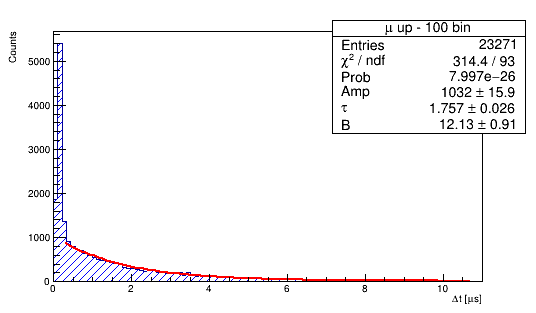
\includegraphics[width=\linewidth]{lifetime/up_final}
		\caption{Up decays.}\label{subfig:final_up}
	\end{subfigure}\hfill
	\begin{subfigure}{.5\linewidth}
		\centering
		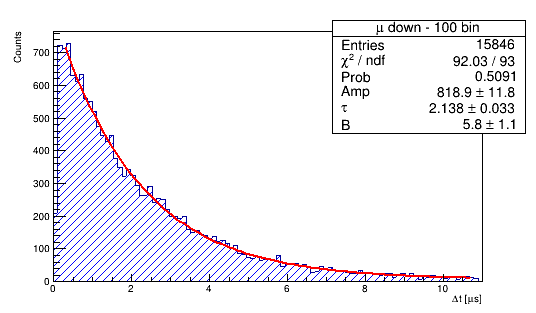
\includegraphics[width=\linewidth]{lifetime/down_final}
		\caption{Down decays.}\label{subfig:final_down}
	\end{subfigure}
	\caption{Muon decay time histogram fitted with the single exponential model \eqref{exp}.}\label{fig:final}
\end{figure}
Histograms displayed in Figure \ref{fig:final} have been fitted with the single exponential model \eqref{exp} hence, down decay results (see Figure \ref{subfig:final_down}) are comparable to what has been obtained by means of the MC discussed above.

The low $p$-value in Figure \ref{subfig:final_up} is a clear sign that these observed data do not adapt to the model, while the observed down decays do (see Figure \ref{subfig:final_down}) since the observed $p$-value is about $51\,\%$. The reason of these behaviors will be investigated in Section \ref{sec:syst}. However, the estimated 
\begin{equation}
\tau=2.138\pm\SI{0.033}{\micro\second}
\end{equation}
is compatible with the nominal value estimated in \ref{tauMC} by means of the MC procedure.

\subsection{$\mu^\pm$ lifetime estimation}
Data referred to down decays have been fitted with a double exponential model too:
\begin{equation}\label{eq:model2exp}
N\left(\Delta t\right) = N_0\left(f_{\mu^+}\cdot e^{-\Delta t/\tau^+} + f_{\mu^-}\cdot e^{-\Delta t/\tau^-}\right)+B
\end{equation}
where $\tau^+$ ($\tau^-$) has been fixed, in order to estimate the $\mu^-$ ($\mu^+$) lifetime. The fractions $f_{\mu^+}$ and $f_{\mu^-}$ are fixed parameters during the fit procedure, but several fits are performed by varying them according to their uncertainties \cite{charge}, in order to keep track of the systematic error.

$\tau^+$ and $\tau^-$ fit results (obtained by employing the nominal $\mu^\pm$ fractions) are shown in Figure \ref{subfig:taup} and \ref{subfig:taum}, respectively.\\
\begin{figure}[!htp]
	\centering
	\begin{subfigure}{.5\linewidth}
	\centering
	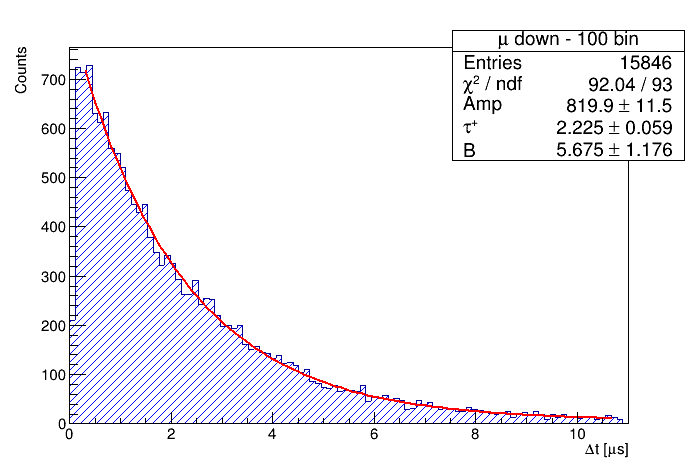
\includegraphics[width=\linewidth]{lifetime/tauplus}
	\caption{$\tau^+$ estimation in down decays.}\label{subfig:taup}
\end{subfigure}\hfill
\begin{subfigure}{.5\linewidth}
	\centering
	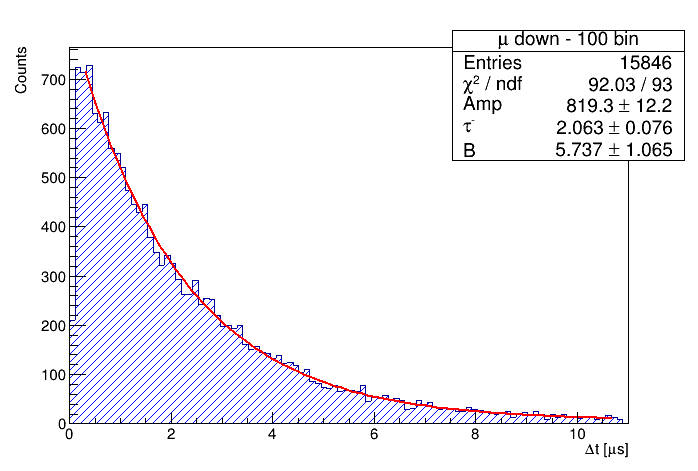
\includegraphics[width=\linewidth]{lifetime/tauminus}
	\caption{$\tau^-$ estimation in down decays.}\label{subfig:taum}
\end{subfigure}
\caption{Down decays fitted with the double exponential model \eqref{eq:model2exp}.}\label{fig:taupm}
\end{figure}

\noindent The final results are
\begin{equation}
\tau^- = \left[2.0628 \pm 0.0595\,(stat) \pm 0.0003\,(syst)\right]\,\si{\micro\second} 
\end{equation}
and
\begin{equation}
\tau^+ = \left[2.2251 \pm 0.0759\,(stat) \pm 0.0002\,(syst)\right]\,\si{\micro\second} 
\end{equation}
We found that the estimated $\mu^\pm$ lifetimes are compatible with the nominal values $\tau^- = \SI{2.026}{\micro\second}$ and $\tau^+ = \SI{2.197}{\micro\second}$.


\section{Systematic errors analysis}\label{sec:syst}

\subsection{Veto windows}
As previously observed in Subsection \ref{subsect::results}, it is evident that different behaviors between up and down triggered decays occur. This difference can be explained in terms of the unequal discriminator time-widths chosen for the detectors. Due to the considerations explained in Subsections \ref{discriminator} and \ref{obs}, the discriminator time-windows selected for the final measurement have been set to values reported in Table \ref{window_meas}.
\begin{table}[!htp]
	\centering
	\begin{tabular}{cc}
		\toprule
		Detector	&	Time-window $(\si{\nano\second})$ \\
		\midrule
		\emph{Cerbero}	&	$57.9$ \\		
		\emph{Minosse}	&	$40.0$ \\
		\emph{Caronte}	&	$40.0$ \\
		\bottomrule		
	\end{tabular}
	\caption{Discriminator output time-windows.}
	\label{window_meas}
\end{table}
Actually, in order to guarantee a proper coincidence operation between signals in \texttt{AND} mode, the \emph{vetoed signal} width should be large enough to include the other ones.
\begin{figure}[!htp]
	\centering
	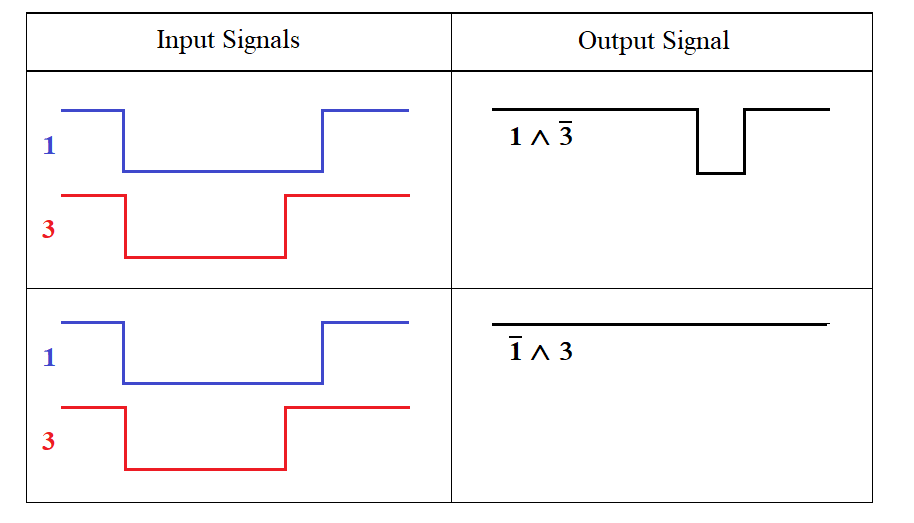
\includegraphics[width=0.75\linewidth]{lifetime/fig_paint}
	\caption{Veto signal time-width impact in \texttt{AND} coincidences. Since pulse 1 is longer than signal 3, when STOPs are vetoed by the latter wrong $1 \land \bar{3}$ STOPs occur, instead if coincidences are vetoed by signal 1, wrong $\bar{1} \land 3$ STOPs are not generated. This fact explains the differences observed between the up and down decay events.}
	\label{vetowindow}
\end{figure}
Figure \ref{vetowindow} shows how the different choices for the discriminator time-windows explain the results obtained for up and down decays, in fact, up decays are triggered by $1 \land \bar{3}$ STOP events but, since \emph{Caronte}'s time-width is $\sim \SI{18}{\nano s}$ shorter than the \emph{Cerbero} one, veto signal 3 does not cover completely signal 1. Therefore, when \emph{Caronte} signal ends, the \emph{Cerbero}'s one goes on and a wrong $1 \land \bar{3}$ STOP signal is generated. This happens systematically for all events in the upper scintillator because of the shorter veto signal width, thus, muons which cross all of the three detectors can generate wrong $1 \land \bar{3}$ STOP signals for the upper scintillator, spoiling the corresponding dataset.

On the other hand, it is clear that this problem does not arise for down decay events since \emph{Cerbero}'s veto width is longer than \emph{Caronte} output duration, hence wrong $\bar{1} \land 3$ STOPs are not generated.\\

As described in Subsection \ref{obs}, it is clear that restricting \emph{Cerbero} time-width from $\SI{80.0}{\nano\second}$ to $\SI{57.9}{\nano s}$ fake coincidences effects were reduced but not completely prevented, since false STOPs were generated in any case. 
\emph{A posteriori}, what should be done is enlarging \emph{Caronte} and \emph{Minosse}'s time-windows making them equal to the \emph{Cerbero}'s one, in order to prevent both \emph{Cerbero} noise fluctuations and false STOPs coincidences.\\

In conclusion, it is possible to declare that data collected as \emph{up decays} are not properly caused by real decay events, instead they are completely corrupt by wrong STOP signals, covering the effects of the real up decays.\\

Concerning the rate of events, the observed value equal to $\SI{0.06}{\hertz}$ is attenuated by the detectors efficiency with respect to the nominal rate. This effect is dominated by the less efficient \emph{Cerbero}, due to \emph{Caronte} and \emph{Minosse} $\varepsilon$ larger than $0.99$. Furthermore, we expect that the rate of START events is not damaged by the choice of \emph{Cerbero}'s veto window, indeed STARTs are given by the coincidence $1 \land 2 \land \overline 3$, but $1 \land 2 $ restricts the width up to \emph{Caronte}'s time-window, which is the same of the vetoed signal 3.\\

Moreover, the upper scintillator STOPs are systematically in advance because of the passage of $\mu^{\pm}$ which are recognized as (wrong) STOPs notwithstanding they are muons that cross all of the three scintillators with a rate equal to $\SI{40}{\hertz}$. This is the reason why when considering up decays, the first bins are highly populated.

%It is possible to notice that the measured rate of events of $\SI{0.06}{Hz}$ is less than expected due to the choice of non optimal working conditions for the detectors. In fact, the choice of increasing \emph{Cerbero}'s threshold voltage in order to reject background events entails a lack in efficiency for \emph{Cerbero}. Since events are triggered by coincidences in which the passage or not of particles in the upper detector is required, the measured rate of events is less than expected because \emph{Cerbero} is less efficient too.  Furthermore, we expect that the rate of START events is not damaged by the choice of \emph{Cerbero}'s veto window. In fact, since STARTs are given by the coincidence $1 \land 2 \land \overline 3$, the coincidence $1 \land 2$ restricts the width up to \emph{Caronte}'s time-window, which is the same of the vetoed signal $\overline 3$.
%Moreover for the upper scintillator STOPs are systematically in advance because of the passage of $\mu^{\pm}$ which are recognized as (false) STOPs notwithstanding they are muons that cross the three scintillators with rate $\SI{40}{Hz}$, and not real STOPs given by $e^{\pm}$ which are emitted toword the upper scintillator. This is the reason why when considering decay events in the upper scintillator the first bins are higly popolated, since $\SI{40}{Hz}$ muons false STOPs are temporally closer to START signal respect to the true ones.


\subsection{Pulls analysis}

In order to study the presence of possible systematic under/over-estimations which affect our measures the \emph{pull method} is employed. For a random variable $x$ with mean $\mu$ and width $\sigma$ the pull is defined as 
\begin{equation}
pull = \frac{ x - \mu }{\sigma}
\end{equation} and is clearly distributed as a standard Gaussian with mean zero and unit width \cite{pull}.
\begin{figure}[!htp]
	\centering
	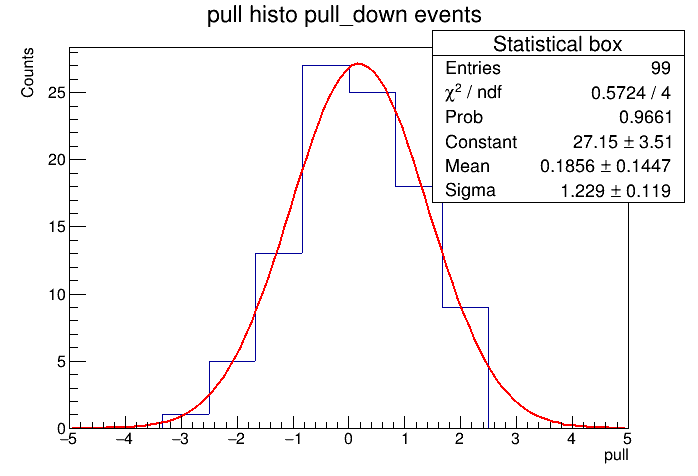
\includegraphics[width=0.6\linewidth]{lifetime/pull_down}
	\caption{Pulls distribution for down scintillator dataset.}
	\label{fig:a}
\end{figure}
Considering the histogram obtained from our dataset the pull corresponding to each bin can be defined as
\begin{equation}
pull_i = \frac{N_{i} - f(\Delta t_{i})}{\sqrt{N_{i}}}
\end{equation}
where $N_i$ is the content of the $i$-bin and $f(\Delta t_{i})$ is the fit function evaluated in the bin $i$.\\

Figure \ref{fig:a} shows the pulls distribution for the down decay dataset. Notice that the mean value of the Gaussian distribution is badly estimated because of the poor binning of the histogram. The discrepancy between the Gaussian mean value and zero is within $1.28 \sigma$ for down decay events, hence, computing the normalized deviation $t$ and fixing a significance level of $5 \%$ it is possible to conclude that down decay events lifetime measures are not \emph{biased}, since $P(t > 1.28) \sim 7\%$.

